
\section*{Problema P6.21}

\renewcommand*\thesection{6.21}
\numberwithin{equation}{section}

\begin{center}
    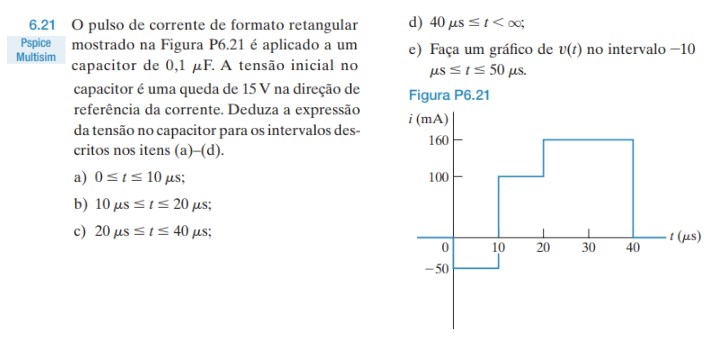
\includegraphics[scale=1.0]{P6.21.jpg}
\end{center}

\subsection*{(a), (b), (c), (d)}


Sabemos que a tensão em um capacitor de capacitância $C$ é dada por

\begin{equation}\label{eq:6.21.1}
    v(t) = V_0 + \frac{1}{C} \int_{t_i}^{t_f} i(t) \,dt
\end{equation}

Usando a figura, e aplicando \eqref{eq:6.21.1} nos intervalos correspondetes ao enunciado, temos

\[ v(t) =
    \begin{cases}
        15 + \frac{1}{C} \int_{0}^{t} (-50 \un{mA}) \,dt,            & 0 \leq t \leq 10 \;\mu\textrm{s}  \\
        \noalign{\vskip9pt}
        \frac{1}{C} \int_{10 \;\mu\textrm{s}}^{20 \;\mu\textrm{s}} (100 \un{mA}) \,dt,    & 10 \leq t \leq 20 \;\mu\textrm{s} \\
        \noalign{\vskip9pt}
        L \cdot (-4), & 20 \leq t \leq 40 \;\mu\textrm{s} \\
        \noalign{\vskip9pt}
        0,            & t > 40 \;\mu\textrm{s}
    \end{cases}
    =
    \begin{cases}
        10 \un{V},            & 0 \leq t \leq 10 \;\mu\textrm{s}  \\
        \noalign{\vskip9pt}
        10 \un{V},    & 10 \leq t \leq 20 \;\mu\textrm{s} \\
        \noalign{\vskip9pt}
        L \cdot (-4), & 20 \leq t \leq 40 \;\mu\textrm{s} \\
        \noalign{\vskip9pt}
        0,            & t > 40 \;\mu\textrm{s}
    \end{cases}
\]

Além disso, temos que a potência no indutor é dada por





